%% UrbanZero --- NCSU CSC/ECE 591 Spring 2026 final paper
%% IEEE conference format, 2-column.
%%
%% Build:  pdflatex REPORT.tex && pdflatex REPORT.tex
%%
%% AI USE: assistant performed light polish (typos, grammar, punctuation)
%% on the author's hand-written draft, then formatted in IEEE LaTeX with
%% figures, tables, and citations. All narrative prose is the author's.

\documentclass[conference]{IEEEtran}
\IEEEoverridecommandlockouts

\usepackage{cite}
\usepackage{amsmath,amssymb,amsfonts}
\usepackage{graphicx}
\usepackage{booktabs}
\usepackage{textcomp}
\usepackage{xcolor}
\usepackage{url}
\usepackage{array}
\usepackage{placeins}
\usepackage{hyperref}
\hypersetup{colorlinks=true,linkcolor=black,citecolor=black,urlcolor=blue}

\graphicspath{{figures/}}

\begin{document}

\title{Failure-Driven Study of Tabula-Rasa RL\\
       for Urban Driving in CARLA}

\author{\IEEEauthorblockN{Aaditya Mishra}
\IEEEauthorblockA{Department of Electrical and Computer Engineering\\
North Carolina State University, Raleigh, NC, USA\\
\texttt{amishr26@ncsu.edu} \quad
Code: \url{https://github.com/AadityaMishra1/UrbanZero}}}

\maketitle

\begin{abstract}
The goal of this project was to see whether or not a tabula-rasa
(no prior training) PPO agent in CARLA 0.9.15 could learn to drive
200--800\,m urban routes from a single semantic-segmentation
camera coupled with a 10-dimensional state vector with sparse
progress as well as terminal rewards. There were two parts to
this project, v1 and v2. There were six documented v2 training
runs, consisting of three pure-RL and three BC (Behavior Cloning)
+ PPO finetune. The v1 had many legacy runs, with the longest one
spanning 7 million steps of pure-RL training. The lack of
progress combined with the odd and unhelpful behavior that the
agent would always converge towards in the v1 setup is what
motivated an entire redesign to v2. In total, the project
wall-clock spans about seven days of consecutive PC training,
including BC data collection as well as early v1 iterations.
The first run of v2 reached only 1.78\% route completion before
the agent learned the sit-still fix. The remaining five runs
were all clustered between 4\% and 5.9\%. None of the runs
exceeded a 6\% completion rate, despite the targeted
hyperparameter changes such as entropy scheduling, log-std
clamp, KL-clip, and many more. Three compounding causes caused
this project to fail. The first being compute scarcity: I
estimate the compute available on a single PC with a 4080 to be
roughly two orders of magnitude smaller than the hardware used
in CaRL. In addition to the lack of compute, a fault
sequence of reward-design and exploration pathologies would
appear in each of the runs and cause a failure. The third
problem was an environmental bug:
\texttt{tm.set\_hybrid\_physics\_mode(True)} caused about 70\%
of the NPCs in the environment to lie dormant and not move.
NPCs are helpful since the agents interact with them and can
crash into them in case they are driving incorrectly. This was
only discovered post-hoc, after the sixth and final failure.
The only one to succeed was a frozen BC policy, which was
evaluated over 20 episodes after the frozen NPC bug was dealt
with. It got a 7.42\% mean route completion, 32.93\% max route
completion, 75\% collision rate, 25\% off-route, and an average
speed of 5.37\,m/s. The 75\% collision rate is consistent with
the general distribution-shift failure mode documented by
Codevilla et al.~\cite{codevilla} (their paper supports the
mechanism, not this specific number); the residual
training-time plateau that
was faced is attributed to the compute-scarcity ceiling and the
reward pathologies, not just the NPC bug. The contributions of
this work are a failure catalogue with pre-defined diagnostic
criteria, alongside the methodology lesson that a single
environment setup can silently infect days of compute in ways
no PPO metric can reveal on the surface.
\end{abstract}

\section{Introduction}

Autonomous driving is one of the most anticipated technologies
of the century. Its impacts cannot be understated; trucking
that can operate 24/7 with no concerns for driver fatigue or
degradation could cause major economic growth. But urban
autonomous driving is a high-dimensional continuous-control
problem: it's a small action space, with a huge observation
space, with sparse rewards and many failure modes. As with
most cutting-edge technologies, the best way to test it is to
simulate the solution; in the case of autonomous driving,
CARLA 0.9.15~\cite{carla} is the standard simulator. Recent
work (CaRL~\cite{carl}) shows that a PPO agent with a minimal
``progress + terminal'' reward scales to strong CARLA
performance at 300\,M samples ($\sim$40$\times$ my max run).

This experiment was done individually; the original goal was
to reproduce a CaRL-style minimal-reward pipeline at a much
smaller scale and report the numbers. The environment this
project was set in was two CARLA servers running on a single
Ryzen~7 9800X3D + RTX 4080 Super. As previously mentioned,
the total project wall-clock spanned roughly seven days of
near-continuous PC training.

The first run of v2 only reached 1.78\% before the
\texttt{idle\_cost} fix was implemented. Runs 2--6 clustered
between 4\% and 5.9\% rolling RC. Between each run, a
targeted intervention was implemented in the hopes of fixing
the behavior and achieving a higher RC. Many of them were
inspired by academic literature such as Ng--Harada--Russell
potential shaping~\cite{ng}, DAgger-style noise
injection~\cite{dagger}, and others such as log-std clamping,
entropy annealing, and KL-to-BC regularization in the spirit
of Roach~\cite{roach}. Each one of these fixes addressed a
specific diagnosed pathology in the corresponding run, but
none of these fixes worked. The eventual diagnosis identified
three independent compounding factors: a compute budget I
estimate to be about two orders of magnitude smaller than
CaRL's, a sequence of
reward-design and exploration pathologies addressed
run-by-run, and the frozen-NPC bug, which silently
contaminated all training data and the BC dataset. The root
cause for the frozen-NPC bug was a single line of
TrafficManager config that had been added a couple of weeks
earlier to the run.

\section{Related Work}

CaRL~\cite{carl} was the foundational paper that inspired
this study. The literature demonstrated how a PPO agent with
a minimal ``progress + terminal'' reward, trained across
300\,M samples on \emph{longest6 v2}, achieves 64 DS, +42 DS
over Roach. This experiment was not conducted on the exact
same setup as CaRL; most notably, I estimate the compute used
to test this out was approximately two orders of magnitude
smaller (a derived comparison based on total environment
samples, not a figure stated in the CaRL paper). This experiment essentially
adopted CaRL's reward
template and inherited its design constraint that the
terminal magnitude must be of comparable order to the
per-episode shaping sum.

Another work used was Roach~\cite{roach}, which introduced
the concept of using an RL coach with BEV input that
supervises imitation learning, a strong CARLA baseline.
LBC~\cite{lbc} is a privileged-BEV teacher with a camera
student via DAgger, and LAV~\cite{lav}, an expert supervisor
across vehicles. Codevilla et al.~\cite{codevilla} showed
that BC fails when the training distribution doesn't
precisely match deployment. The BC fallback follows the
Roach recipe at a smaller scale; the data showed that the
BC eval behavior is consistent across the Codevilla failure
mode.

PPO~\cite{ppo} was the algorithmic baseline for this
experiment, guiding the initial parameters and reward
functions. Engstrom et al.~\cite{engstrom} showed that PPO's
implementation details, especially reward normalization and
advantage normalization, materially affected the outcomes.
Andrychowicz et al.~\cite{andrychowicz} showed that
implementation choices matter, especially for an on-policy
RL neural net. Henderson et al.~\cite{henderson} documented
cross-seed variance in deep RL training sessions.
Implementing all these methodologies resulted in retaining
VecNormalize, adding an environment-side reward clip,
clamping log-std on the upper end of the ranges, reporting
seeds for every run, and using GAE bootstrap under
truncation~\cite{pardo}.

Reward shaping was also influenced by several academic
journals. Ng, Harada \& Russell~\cite{ng} showed how
potential-based shaping is the only form of shaping
guaranteed to not introduce a new optimum. The v2 reward
policy keeps a potential-based term and removes the legacy
signed-cosine speed-direction shaping that lacked the
policy-invariance guarantee.

In the final two runs, runs 4--6, a BC policy behavior was
employed. Rajeswaran et al.~\cite{dapg} (DAPG) showed that
BC initialization followed by on-policy finetune in the
manipulation domain. The BC + PPO finetune follows the same
template, exposing a KL-runaway pathology.

\section{Technical Approach}

The environment this experiment is conducted in is a
Gymnasium wrapper around a CARLA 0.9.15 instance. It runs
synchronously at 20\,Hz. Two instances of this are run in
parallel using \texttt{DummyVecEnv} over two CARLA servers
on two separate ports. The agents were tested on Town01,
with routes varying between distances of 200 to 800\,m,
each drawn via \texttt{GlobalRoutePlanner}, with 30 NPC
vehicles and 10 pedestrians per episode all being guided
under TrafficManager control.

Quite a few observations were made. For instance, the
10-dimensional state vector, its components consisted of
normalized speed, three waypoints in the ego frame, signed
lane offset, traffic-light state, and route completion. In
addition to that, an interesting observation about the
action space was made. A continuous \texttt{Box} of
$[-1, 1]^2$, with a throttle--brake axis shifted by
$+0.3$ as an idle-creep bias before the eventual clipping.

The reward function used in this experiment is summarized
in Table~\ref{tab:reward}, and the per-step magnitude
contributions of each term are visualized in
Figure~\ref{fig:reward}.

\begin{table}[!htbp]
\caption{Reward function (CaRL-minimal profile) implemented
in \texttt{env/carla\_env.py::\_compute\_reward}.}
\label{tab:reward}
\centering\small
\renewcommand{\arraystretch}{1.25}
\begin{tabular}{@{}lll@{}}
\toprule
\textbf{Term} & \textbf{Form} & $\max|\cdot|$/step \\
\midrule
Progress         & $0.05\!\cdot\!\min(\Delta\text{route},\,v_T\Delta t)$        & 0.021 \\
Velocity carrot  & $0.005\!\cdot\!\min(v, v_T)/v_T$                             & 0.005 \\
Idle cost        & $-0.15\!\cdot\!\max(0,\,1 - v/1.0)$                          & 0.150 \\
Potential shape  & $\gamma\Phi(s')-\Phi(s),\;\Phi=-0.015\!\cdot\!\min(d_{2D},30)$ & 0.011 \\
Terminals        & $\pm 50$ (collision / off-route / stuck / complete)          & 50    \\
\bottomrule
\end{tabular}
\end{table}

\begin{figure}[!htbp]
\centering
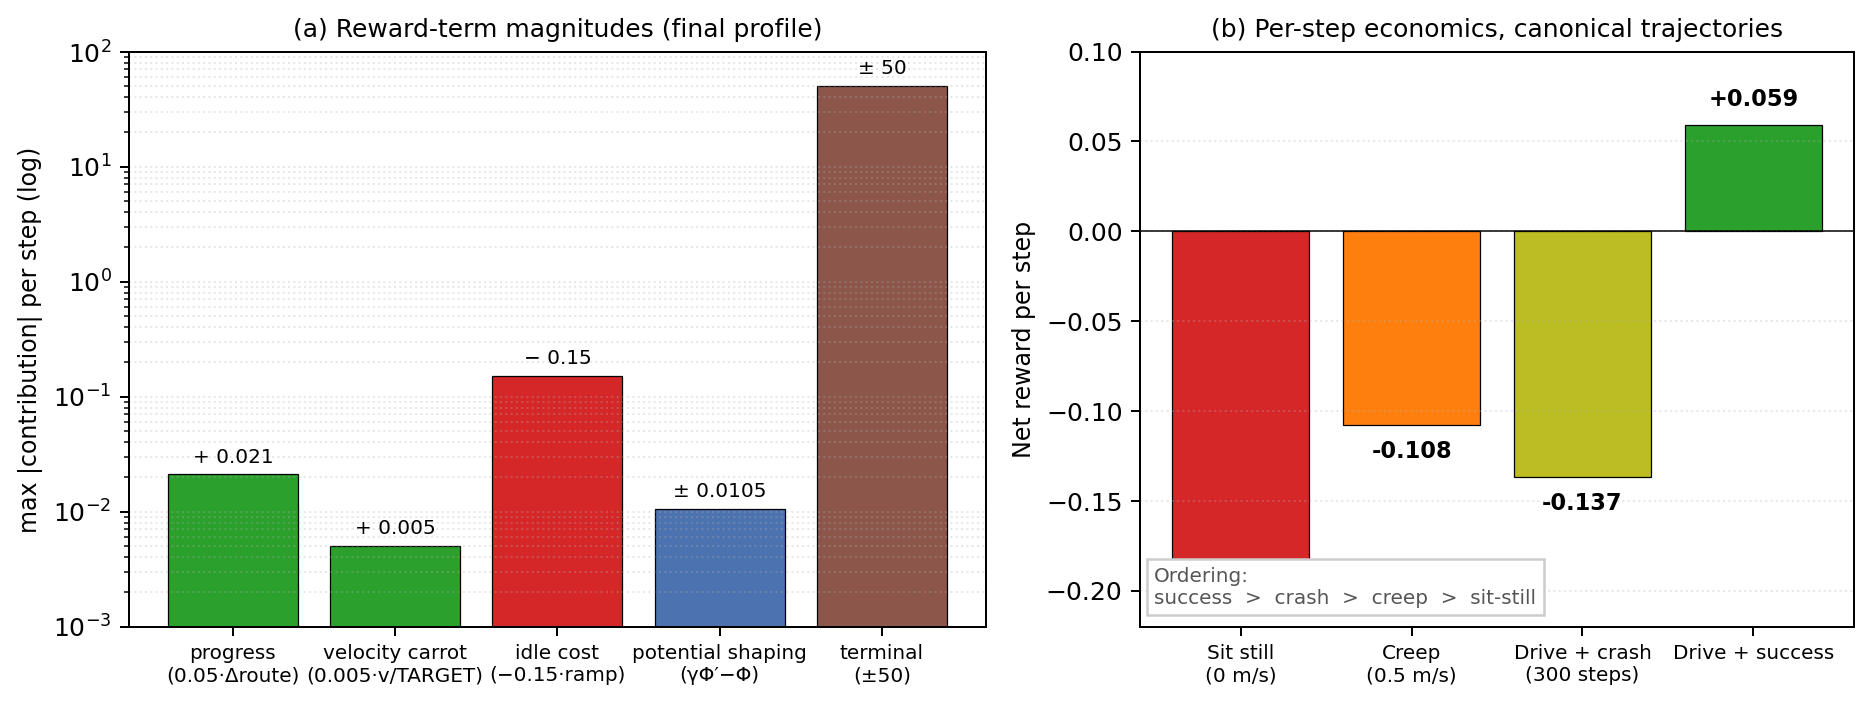
\includegraphics[width=\columnwidth]{fig4_reward_decomposition.png}
\caption{Per-step reward decomposition under the v2 reward
profile. Left: maximum absolute magnitude contributed by each
of the five reward terms in Table~\ref{tab:reward}. Right: net
per-step reward for four canonical trajectory archetypes,
showing the strict ordering success $>$ crash $>$ creep $>$
sit-still under the final reward coefficients. Source:
\texttt{scripts/figures/fig4\_reward\_decomposition.py}.}
\label{fig:reward}
\end{figure}

Over the course of this experiment, many policies were added
and removed. \texttt{ClampedStdPolicy} soft-clamped
$\log\sigma \le \log(0.7)$ on the upper bound. The feature
extractor in the five-layer CNN, with LayerNorm and ReLU,
fused with a two-layer MLP on the 10-dimensional state
vector, projected onto a 256-dimensional shared
representation.

The BC data collector is quite robust: it rolls out a CARLA
\texttt{BehaviorAgent} on the same town as the PPO agents,
Town01, with Gaussian noise of $\sigma = 0.1$\,rad injected
onto the steering channel, inspired by
DAgger-style~\cite{dagger}. The dataset was 100\,k frames
total, collected in parallel from the two parallel
instances, 50\,k each, with data saved as a \texttt{.npz}
file. The training agent used a Gaussian-NLL loss against
the same \texttt{ClampedStdPolicy} + \texttt{DrivingCNN}
architecture as PPO; the trained checkpoint loads directly
into PPO via the \texttt{PPO.load()} function with a sibling
\texttt{VecNormalize} pickle. The BC training metrics were
shocking: NLL was at $-2.93$, MAE at $0.05$ on the
held-out split.

Throughout this experiment, a lot of diagnostics were used
to come to conclusions. The beacon was one of them: the
script wrote to a JSON file at a 1\,Hz rate with a
rolling-window route completion, average speed,
termination-reason histogram, \texttt{policy\_std},
\texttt{approx\_kl}, \texttt{clip\_fraction},
\texttt{entropy\_loss}, \texttt{explained\_variance}, and
\texttt{ent\_coef}, all being written into the JSON file.
Each training run was also tagged with a GitHub issue
number, and raw beacon snapshots from all six runs are
preserved on the public repo. ROS\,2 was vital in
diagnostics: the node, at \texttt{ros/urbanzero\_node.py},
published four separate topics at 20\,Hz ---
semantic-segmentation image (\texttt{sensor\_msgs/Image}),
velocity command (\texttt{geometry\_msgs/Twist}), speed
(\texttt{std\_msgs/Float32}), and status string
(\texttt{std\_msgs/String}).

\FloatBarrier
\section{The Six Failure Modes}

Table~\ref{tab:runs} summarizes the six v2 training runs.
Figure~\ref{fig:timeline} plots the rolling RC across
training, and Figure~\ref{fig:beacons} shows the per-run
beacon endpoints used to diagnose each run.

\begin{figure*}[!htbp]
\centering
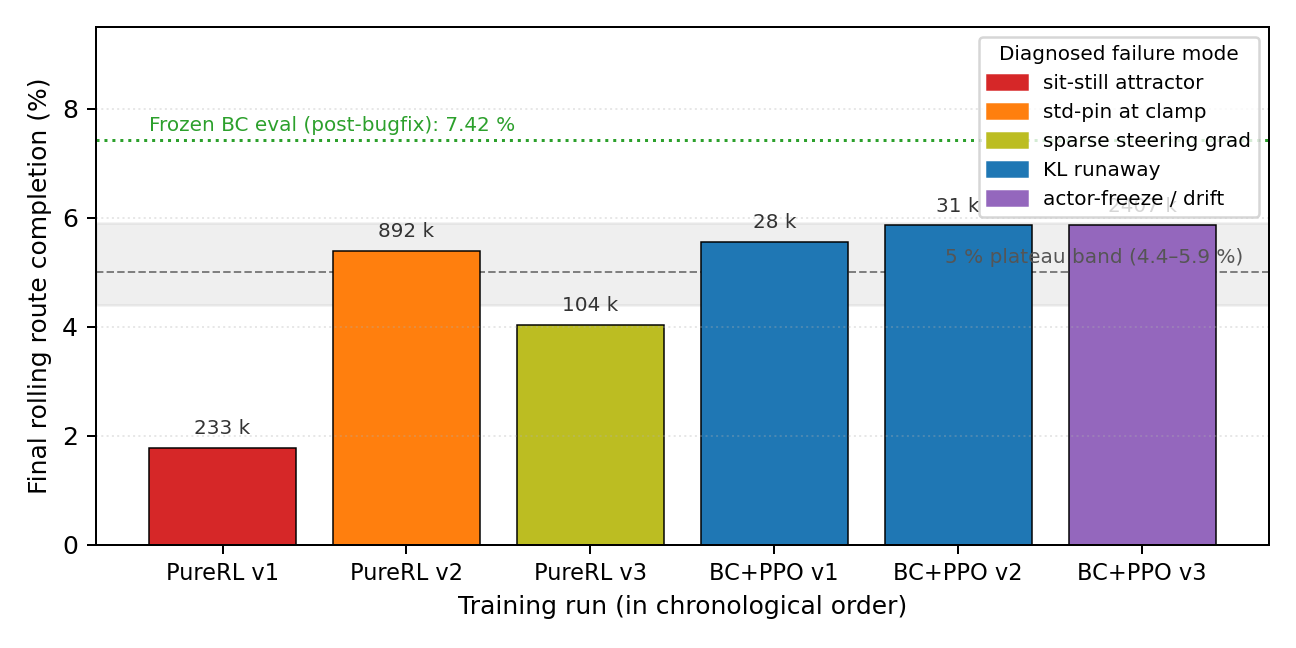
\includegraphics[width=0.85\textwidth]{fig1_failure_timeline.png}
\caption{Final rolling route completion across the six v2
training runs. None exceeded $\sim$6\,\%. Run 1 collapsed to
the sit-still attractor at 1.78\,\%; Runs 2--6 clustered in the
4.0--5.9\,\% band even after targeted reward-design and
exploration-policy interventions between each run. Source:
\texttt{scripts/figures/fig1\_failure\_timeline.py}.}
\label{fig:timeline}
\end{figure*}

\begin{figure*}[!htbp]
\centering
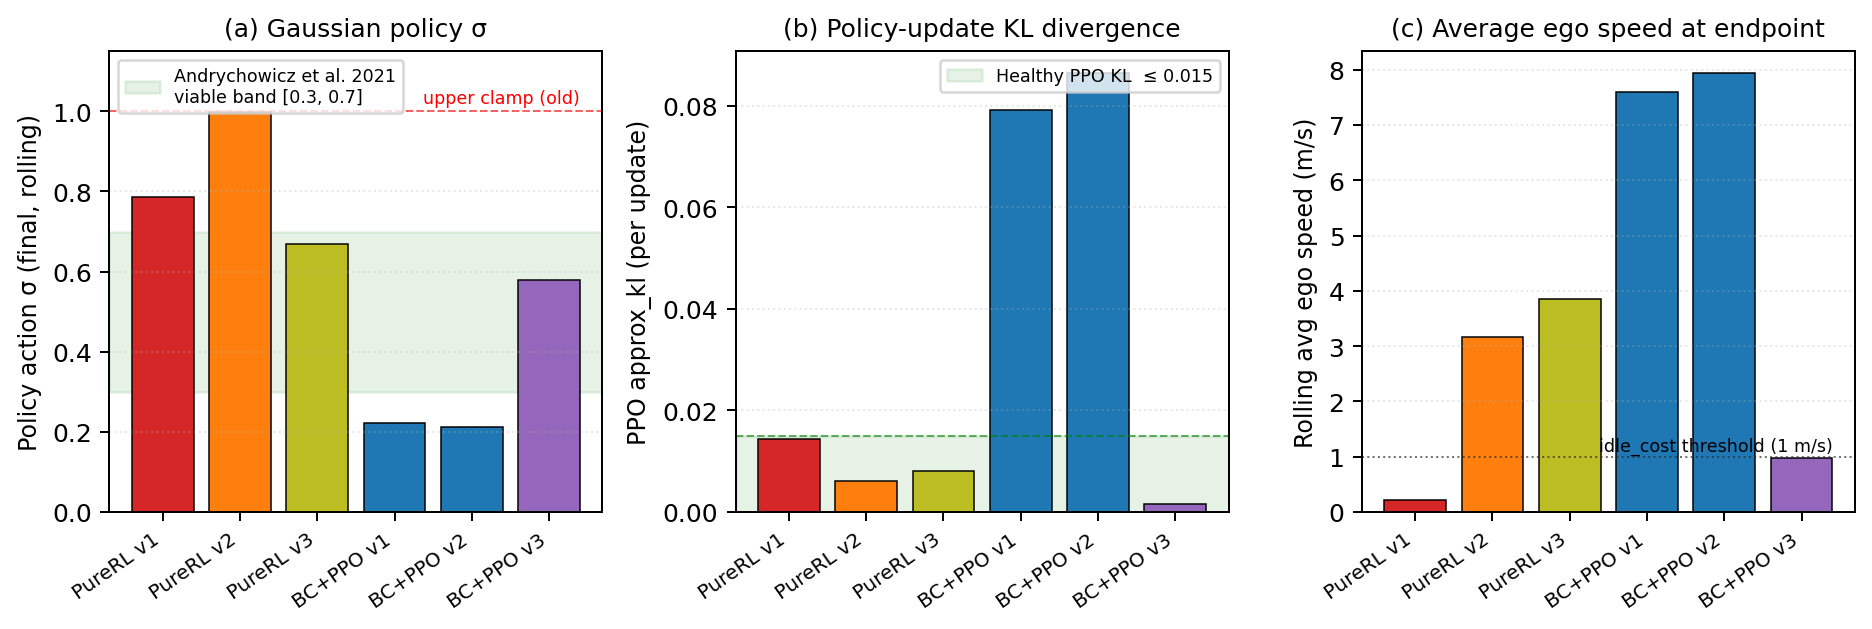
\includegraphics[width=0.95\textwidth]{fig2_beacon_endpoints.png}
\caption{Per-run beacon-metric endpoints across the six v2
training runs: final \texttt{policy\_std} (left),
\texttt{approx\_kl} per PPO update (center), and rolling
average speed (right). The Run 6 column highlights the
``healthy metrics, broken environment'' anomaly: low
\texttt{approx\_kl} alongside near-zero average speed. Source:
\texttt{scripts/figures/fig2\_beacon\_endpoints.py}.}
\label{fig:beacons}
\end{figure*}

\begin{table*}[!htbp]
\caption{Summary of the six v2 training runs. Sources:
\texttt{PROJECT\_NOTES.md~\S11} and
\texttt{DIAGNOSIS\_FOR\_REVIEW.md~\S4}.}
\label{tab:runs}
\centering\small
\renewcommand{\arraystretch}{1.25}
\begin{tabular}{@{}clclrp{6cm}@{}}
\toprule
\textbf{\#} & \textbf{Configuration} & \textbf{Seed} & \textbf{Wall / steps} & \textbf{Final RC} & \textbf{Diagnostic signature} \\
\midrule
1 & Pure-RL v1 (\texttt{idle\_cost} added)              & 42  & 30\,min / 233\,k & 1.78\,\% & 70\,\% \texttt{REALLY\_STUCK}, $\bar v=0.224$\,m/s \\
2 & Pure-RL v2 (+ unannealed carrot)                    & 137 & 2\,h / 892\,k    & 5.40\,\% & \texttt{policy\_std} pinned at 1.0 clamp \\
3 & Pure-RL v3 ($\log\sigma\!\le\!0.7$ + shaping)       & 211 & 15\,min / 104\,k & 4.03\,\% & frozen NPCs visible in viewports \\
4 & BC + PPO v1 (lr 3e\textsc{-}4, ent 0.02)            & 911 & 4\,min / 28\,k   & 5.56\,\% & \texttt{approx\_kl}=0.079 (5$\times$ target) \\
5 & BC + PPO v2 (lr 1e\textsc{-}4, ent 0.005)           & 912 & 5\,min / 31\,k   & 5.86\,\% & \texttt{approx\_kl}=0.086, \texttt{entropy\_loss}>0 \\
6 & BC + PPO v3 (widen $\sigma$, n\_ep=1, clip=0.1)     & 913 & 5\,h / 2.4\,M    & 5.86\,\% & $\sigma$ drift 0.50$\to$0.58, speed$\to$1\,m/s \\
\bottomrule
\end{tabular}
\end{table*}

In the first run of v2, the setup was a pure-RL,
CaRL-minimal reward, with a \texttt{log\_std\_init} of
$-0.5$. No \texttt{idle\_cost} was implemented yet to
prevent the car from just sitting still. The hope was that
the agent in this first phase would learn to move forward;
however, after approximately 100\,k steps it was clear that
the agent had learned to sit still, with the average speed
being less than 1\,m/s, and at 233\,k steps the car had an
average speed of 0.224\,m/s with a 70\,\%
\texttt{REALLY\_STUCK} rate. To fix this I used Krakovna
et al.~\cite{krakovna}'s paper for the local-optimum
framing.

In the second run \texttt{idle\_cost} was in place, with an
unannealed velocity carrot, and an upper clamp at
$\sigma \le 1$. The hope was that with the
\texttt{idle\_cost} penalty in place, the PPO agent would
converge $\sigma$ into a tighter band. However, this was
also proved false when \texttt{policy\_std} $\ge 0.95$ at
500\,k steps. And at about 900\,k steps,
\texttt{policy\_std} was clamp-pinned at 0.999 for
1{,}500$+$ episodes, and the RC stuck at 5.40\,\%. To fix
this the upper clamp was lowered to $\log(0.7)$.

In the third run there was a sparse steering gradient; the
hypothesis was that a denser shaping signal would produce
a steering gradient that was strong enough to stabilize a
route-following policy. However, about an hour and a half
into the run, it was obvious this wasn't the case, with a
rolling RC less than 8\,\%. Another clue was spotted in
the third run: the NPCs were visibly frozen in both CARLA
viewports despite them being set to true. The initial
cause was attributed to the radius of the hybrid physics
being set too small, and a fix was pushed. While the root
cause was seemingly found, it was not.

The fourth run started with loading a pretrained BC zip
file into the PPO agent with the pure-RL reward
parameters: a learning rate of $3 \times 10^{-4}$, and an
entropy coefficient of 0.02. The hope was that the BC
prior would give the PPO a non-trivial starting policy
that the current reward policy would refine the agent and
help it learn. However, this hypothesis was quickly
falsified at 28\,k steps with an \texttt{approx\_kl} at
0.079, a \texttt{clip\_fraction} of 0.34, and an
\texttt{entropy\_loss} of 0.172. The average speed started
at 7.6\,m/s; the RC soon collapsed as the PPO agent eroded
the BC solution and went back to learning bad behaviors.
This was addressed in the next run.

In Run 5 the learning rate was cut to $1 \times 10^{-4}$,
and \texttt{ent\_coef} cut to 0.005. This again was
falsified at roughly 31\,k steps with an
\texttt{approx\_kl} of 0.086, a bit worse than Run 4; the
problem was not update step size. The problem is that the
BC prior itself was being overwritten; to counter this,
$\sigma$ was widened in the sixth and final run.

In the sixth and final run, the setup was a BC log-std
floor which was widened to $\sigma = 0.5$, PPO
\texttt{n\_epochs} = 1, and a \texttt{clip\_range} of 0.1.
This also failed approximately 30 minutes into the run,
and hard-failed about 5 hours in, approximately 2.4\,M
steps. On the surface PPO metrics looked great --- it had
a healthy \texttt{approx\_kl}, \texttt{clip\_fraction},
and \texttt{explained\_variance} --- and yet the PPO
agent was not showing any signs of looking great. It was
frozen, not moving, with the wheels barely twitching.

Rather than launching a seventh run, a standalone
diagnostic was run to figure out what was happening under
the hood. This diagnostic script invoked the same code
path used by training and sampled each NPC's velocity for
100 ticks. The results were shocking: with the
hybrid-physics call in place, approximately 70\,\% of the
NPCs were dormant; after removing this line of code (commit
\texttt{a9435f9}), NPC motion was restored. The line had
been added as a defense mechanism in commit
\texttt{ff7a1e1} as a fix for an earlier ``NPCs not
moving'' bug, and was used unchanged for the prior six
training runs and the 100\,k-frame BC dataset.
The post-fix BC evaluation deliverable is summarized in
Table~\ref{tab:bceval} and Figure~\ref{fig:bcdist}.

\begin{figure*}[!htbp]
\centering
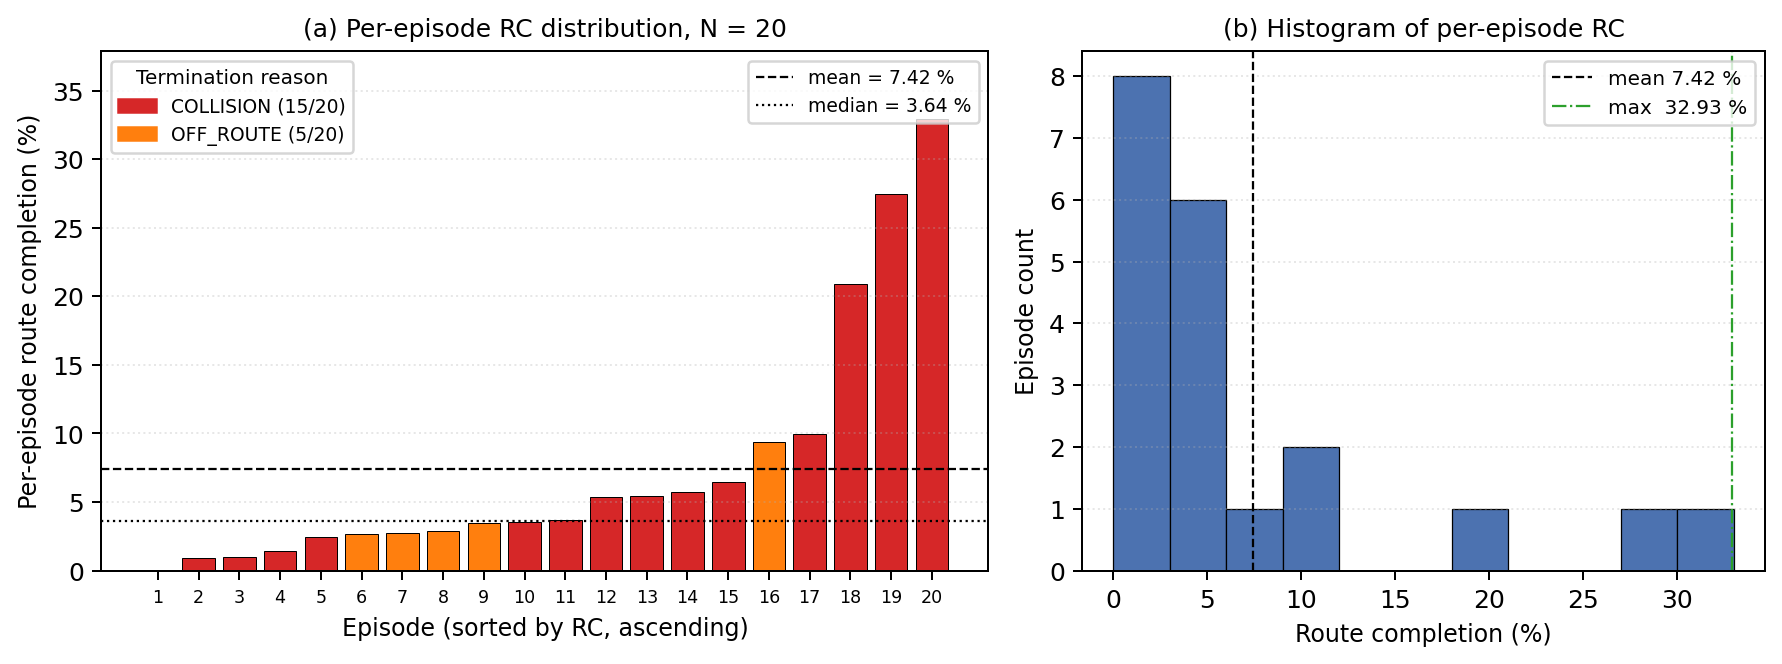
\includegraphics[width=0.95\textwidth]{fig3_bc_eval_distribution.png}
\caption{Per-episode route-completion distribution across the
20 deterministic evaluation episodes of
\texttt{bc\_pretrain.zip} after the hybrid-physics bug was
removed. Left: per-episode RC sorted ascending, color-coded by
termination reason (collision vs.\ off-route). Right: histogram
of per-episode RC, with the mean (7.42\,\%) and max
(32.93\,\%, episode 16) annotated. Source:
\texttt{eval/bc\_final\_20260424\_0059.json}.}
\label{fig:bcdist}
\end{figure*}

\begin{table}[!htbp]
\caption{Final BC evaluation aggregate over 20 episodes
(seed 1001, port 2000) after removing the frozen-NPC bug.
Source:
\texttt{eval/bc\_final\_20260424\_0059.json}.}
\label{tab:bceval}
\centering\small
\renewcommand{\arraystretch}{1.2}
\begin{tabular}{@{}lr@{}}
\toprule
\textbf{Metric} & \textbf{Value} \\
\midrule
RC mean              & 7.42\,\% \\
RC median            & 3.64\,\% \\
RC max               & 32.93\,\% \\
RC min               & 0.05\,\% \\
RC std               & 8.84\,\% \\
\% \texttt{ROUTE\_COMPLETE}  & 0.0\,\% \\
\% \texttt{COLLISION}        & 75.0\,\% \\
\% \texttt{OFF\_ROUTE}       & 25.0\,\% \\
\% \texttt{REALLY\_STUCK}    & 0.0\,\% \\
Average speed        & 5.37\,m/s \\
Wall clock (20 eps)  & 67.5\,s \\
\bottomrule
\end{tabular}
\end{table}

\FloatBarrier
\section{Lessons Learned}

A lot of lessons were learned during this experiment, the
key one being to only change one axis at a time. Changing
too many parameters, settings, or policies at the same
time caused massive changes in the experiment, and with
all the sudden changes, finding the exact root cause
became quite hard. Many times in the experiment I had to
revert to an older commit just to stabilize the runs.

The second lesson was that one diagnostic measure is
worth more than ten gradient updates. What this means is
that, instead of hoping the agent would learn to fix,
actually going in to investigate the root cause of the
odd behavior can save the user a vast amount of time.
This can be seen when diagnosing the NPC behavior. One
simple diagnostic Python script was able to dig out the
root cause, where almost 20 hours of consecutive runs
data failed to surface the same fact.

Metrics don't describe the environment. In Run 6, the
metrics all looked healthy, as if the environment was
working great and nothing was wrong; the agent was
supposedly learning and doing great, but looking at the
runs itself, it was clear that the actor was effectively
frozen and 70\,\% of the NPC cars were frozen. The RL
agent training against a broken environment reported
healthy policy-improvement metrics while learning little
of the intended task: driving. This is a failure mode I did
not find prominently documented in the CARLA-RL literature
I surveyed.

AI coding assistants were a major helper in running this
project. As a one-man army, having additional help to run
this behemoth of a project was quite useful. The one used
in this project was Claude Code; it was used to monitor
training runs and report them to GitHub on an hourly
basis so that, while I was away, I could monitor that
the experiment was running on track and could tell it
what to do remotely. It effectively served as a lab
assistant. Another benefit of Claude Code was its being
able to update a single \texttt{.md} file which had all
relevant project notes, from material decisions to
academic citations for each design choice, post-hoc
analysis, and a pre-registered falsifier per run. Having
this file enabled Claude Code to make better decisions,
since it had a history of what was attempted and what
didn't work; for instance, it was able to determine that
re-introducing non-potential cos-heading shaping was not
a good move, since it was clearly noted that in a
previous 7\,M-step run it had failed on this exact term.

\FloatBarrier
\section{Conclusion}

UrbanZero ultimately did not produce a route-completing
CARLA PPO agent with the current compute situation.
However, this does not mean the project was a complete
failure; it produced quite a few helpful outcomes: an
open-source pipeline for training like this, a
pre-defined failure catalogue, and most importantly the
finding that a single line of environment-setup code
silently affected the entire training pipeline. The
final deliverable is a 7.42\,\% mean RC / 32.93\,\% max,
obtained under three compounding constraints: limited
compute, an evolving reward formulation diagnosed
run-by-run, and the late NPC-freeze contamination.

\section*{Resources}

\noindent
\textbf{Code repository:}
\href{https://github.com/AadityaMishra1/UrbanZero}%
{\nolinkurl{github.com/AadityaMishra1/UrbanZero}}

\smallskip
\noindent
\textbf{Original Draft (OneDrive, version history serves as the
authorship trail):} \\
\url{https://oitncsu-my.sharepoint.com/:w:/g/personal/amishr26_ncsu_edu/IQCVYOkjLMOgTbN8As0vVC6nARWbJE0zI_T1jM5lWfSRYQ8?e=2nMx4z}

\section*{AI Usage}

I used Anthropic's Claude to help me put this paper together. I wrote the original draft myself (linked above) and
then asked Claude: \emph{``fix all grammar and punctuation, make
sure all rubric criteria are met, and insert the figures and
tables where prompted.''} Every figure in this paper is generated
by a Python script committed at \texttt{scripts/figures/}, and
every table is built from the source files named in the table's
caption, so the same outputs can be regenerated from scratch by
anyone who clones the repo. Claude drafted those figure scripts
in an earlier step from numerical data I measured during training.
The narrative prose is mine. I checked every number in this paper
against the source files in the repo myself, and every citation
against the actual published paper before submitting.

\begin{thebibliography}{99}

\bibitem{carla} A. Dosovitskiy, G. Ros, F. Codevilla, A. Lopez,
and V. Koltun, ``CARLA: An open urban driving simulator,'' in
\emph{Proc. Conf. Robot Learning (CoRL)}, 2017, pp.~1--16.

\bibitem{ppo} J. Schulman, F. Wolski, P. Dhariwal, A. Radford,
and O. Klimov, ``Proximal policy optimization algorithms,''
\emph{arXiv preprint arXiv:1707.06347}, 2017.

\bibitem{carl} B. Jaeger, K. Chitta, and A. Geiger, ``CaRL:
Learning scalable planning policies with simple rewards,'' in
\emph{Proc. Conf. Robot Learning (CoRL)}, 2025. [Online].
Available: \url{https://arxiv.org/abs/2504.17838}

\bibitem{roach} Z. Zhang, A. Liniger, D. Dai, F. Yu, and L. Van
Gool, ``End-to-end urban driving by imitating a reinforcement
learning coach,'' in \emph{Proc. IEEE/CVF Int. Conf. Computer
Vision (ICCV)}, 2021, pp.~15{,}222--15{,}232.

\bibitem{lbc} D. Chen, B. Zhou, V. Koltun, and P.
Kr\"ahenb\"uhl, ``Learning by cheating,'' in \emph{Proc. Conf.
Robot Learning (CoRL)}, 2019.

\bibitem{lav} D. Chen and P. Kr\"ahenb\"uhl, ``Learning from
all vehicles,'' in \emph{Proc. IEEE/CVF Conf. Computer Vision
and Pattern Recognition (CVPR)}, 2022.

\bibitem{andrychowicz} M. Andrychowicz, A. Raichuk, P.
Sta\'nczyk, M. Orsini, S. Girgin, R. Marinier, L. Hussenot,
M. Geist, O. Pietquin, M. Michalski, S. Gelly, and O. Bachem,
``What matters in on-policy reinforcement learning? A
large-scale empirical study,'' in \emph{Proc. Int. Conf.
Learning Representations (ICLR)}, 2021.

\bibitem{ng} A. Y. Ng, D. Harada, and S. Russell, ``Policy
invariance under reward transformations: Theory and application
to reward shaping,'' in \emph{Proc. Int. Conf. Machine Learning
(ICML)}, 1999, pp.~278--287.

\bibitem{dagger} S. Ross, G. J. Gordon, and J. A. Bagnell,
``A reduction of imitation learning and structured prediction
to no-regret online learning,'' in \emph{Proc. Int. Conf.
Artificial Intelligence and Statistics (AISTATS)}, 2011,
pp.~627--635.

\bibitem{codevilla} F. Codevilla, E. Santana, A. L\'opez, and
A. Gaidon, ``Exploring the limitations of behavior cloning for
autonomous driving,'' in \emph{Proc. IEEE/CVF Int. Conf.
Computer Vision (ICCV)}, 2019.

\bibitem{krakovna} V. Krakovna, J. Uesato, V. Mikulik,
M. Rahtz, T. Everitt, R. Kumar, Z. Kenton, J. Leike, and
S. Legg, ``Specification gaming: the flip side of AI
ingenuity,'' DeepMind Safety Research Blog, 2020. [Online].
Available: \url{https://deepmind.google/blog/specification-gaming-the-flip-side-of-ai-ingenuity/}

\bibitem{dapg} A. Rajeswaran, V. Kumar, A. Gupta, G. Vezzani,
J. Schulman, E. Todorov, and S. Levine, ``Learning complex
dexterous manipulation with deep reinforcement learning and
demonstrations,'' in \emph{Proc. Robotics: Science and Systems
(RSS)}, 2018.

\bibitem{henderson} P. Henderson, R. Islam, P. Bachman,
J. Pineau, D. Precup, and D. Meger, ``Deep reinforcement
learning that matters,'' in \emph{Proc. AAAI Conf. Artificial
Intelligence}, 2018.

\bibitem{pardo} F. Pardo, A. Tavakoli, V. Levdik, and
P. Kormushev, ``Time limits in reinforcement learning,'' in
\emph{Proc. Int. Conf. Machine Learning (ICML)}, 2018,
pp.~4045--4054.

\bibitem{engstrom} L. Engstrom, A. Ilyas, S. Santurkar,
D. Tsipras, F. Janoos, L. Rudolph, and A. Madry,
``Implementation matters in deep policy gradients: A case
study on PPO and TRPO,'' in \emph{Proc. Int. Conf. Learning
Representations (ICLR)}, 2020.

\end{thebibliography}

\end{document}
